\newpage
\begin{savequote}[108mm]
``Nothing is impossible, the word itself says 'I'm possible''
   \qauthor{Audrey Hepburn}
\end{savequote}
\chapter{Case of study}
\label{chap:Caseofstudy}
\vspace{-2cm}
The rise of FLOSS has caused many organizations and even many governments to consider the possibility of a migration. This chapter will describe some of the successful cases of migration to the use of these types of programs. 
%--------------------------------------------------------------

\section {Zaragoza, Spain}
\label{Zaragoza}

\begin{figure}[H]
\centering
    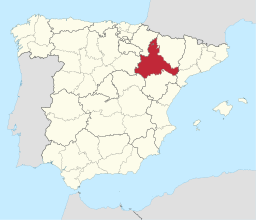
\includegraphics[scale=0.8]{img/Zaragoza.png} 
  \caption{Zaragoza city}
    \end{figure}
Zaragoza is one of the largest cities in Spain; the city itself boasts approximately 5,000 employees who offer a wide range of services to the approximately 660,000 people who reside therein. 

\subsection{AZLinux}

AZLinux is the Linux distribution, based on OpenSuSE, that was created and promoted by the city council of Zaragoza. Since 2003, the promotion and use of  FLOSS by the city has become one of the identifying marks of the Zaragoza City Council, in respect to IT matters.

In 2005, the City Council adopted a motion that urged the city’s local government to promote the use of  FLOSS, especially by all municipal employees. 

\textit{``We have to explain ourselves to users, technicians, public managers and almost every body else. We discovered that fear, uncertainty and doubt are very effective tools to hinder our progress. Fortunately, our politicians promote and support our IT policies to switch to free software. Obtaining and maintaining this political support is crucial to overcome difficulties in the migration process.''}\footnote{Eduardo Romero, computer technician at City of Zaragoza in\url{https://joinup.ec.europa.eu/news/es-zaragozas-move-complete-open-source-desktop-going-plan}}

As a result of this motion, considerable savings have been made in regard to the associated licensing costs that were previously being paid out and expert knowledge has been gained, knowledge being shared with the local community. 
\begin{table}[H] \centering

\begin{tabular}{| c| c |}
\hline
PCs with OpenOffice & +3,000\\\hline
PCs using Linux   & +600  \\ \hline
Free Software      & 100\%  \\ \hline
Servers Using Linux  & 80\% \\ \hline
Computer Literacy Centers & 17   \\
\hline
\end{tabular}
\caption{Zaragoza Implementation of Free Software}
\label{table:Zaragoza implementation}
\end{table}

%MORRRRRE DETILES
In the same year, an agreement was signed with HispaLinux that setup a building dedicated to the promotion and use of   FLOSS within the city; seven years later, this facility is still running and has since become the focal point for all free knowledge related activities and serves as a tele-center for those that have a need of it.

As Table \ref{table:Zaragoza implementation} indicates, the number of those who are utilizing the Linux computer literacy centers and those who have taken advantage of the switch over to FLOSS is far greater than could have been anticipated\footnote{\url{http://www.zaragoza.es/contenidos/sectores/tecnologia/Estrategia-Ciencia-Tecnologia-en.pdf}}.


\subsection{Migration plan}

  The Zaragoza migration took place in three phases. First lightweight applications were transferred, then office operations, and finally the operating system. This method resulted in the least amount of downtime for the business the results of the study found that this migration method was an effective means to perform the migration\footnote{\url{http://www.slideshare.net/slides\_eoi/migracin-a-software-libre-del-escritorio-del-ayuntamiento-de-zaragoza}}.

 \begin{figure}[H]
 \centering
     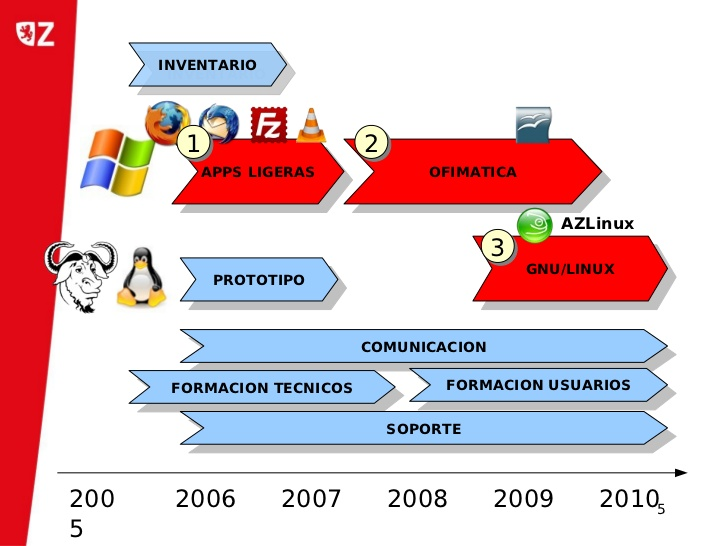
\includegraphics[scale=0.5]{img/desktopplan.jpg} 
  \caption[Migration plan in Zaragoza]{Migration plan for Zaragoza \protect\footnotemark}   
     \label {fig:plan-Zara}
     \end{figure}
     \footnotetext{ Source: \url{http://www.slideshare.net/eduromo/ubuntu-migration-at-zaragoza-city-council-v3}\label{planzaragoza}}
     
     \begin{figure}[H]
     \centering
         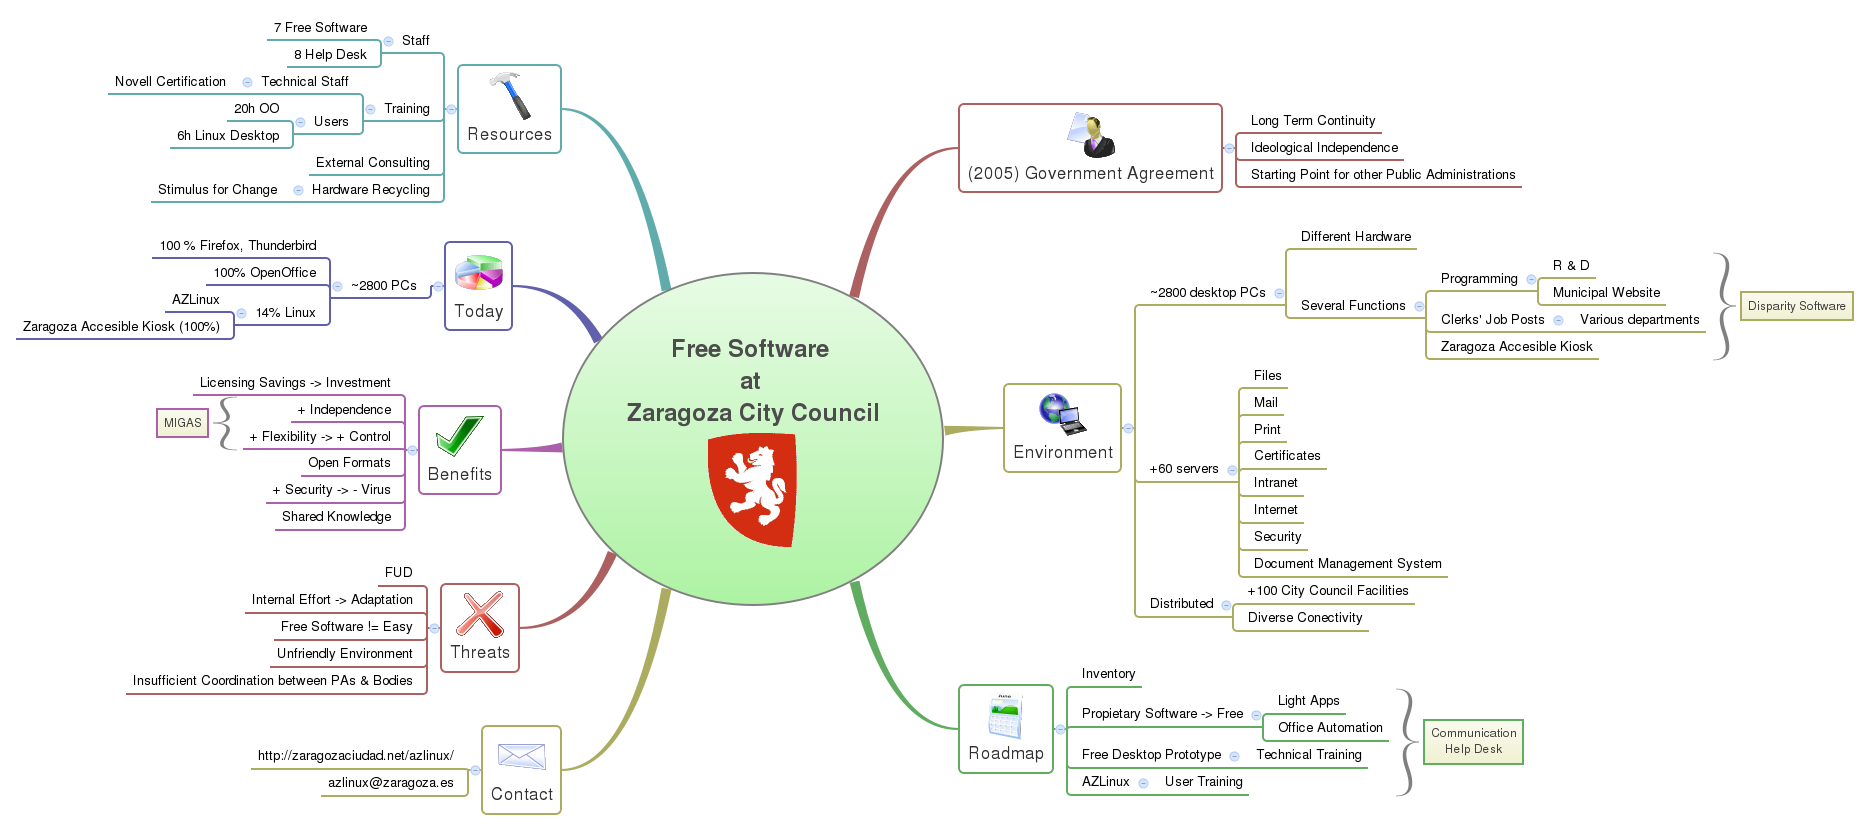
\includegraphics[scale=0.3,angle=90]{img/aytozgz.png} 
       \caption[Free Software at Zaragoza City Council]{Free Software at Zaragoza City Council \protect\footnotemark}
       \label{fig:FsZ}
         \end{figure}
     \footnotetext{Source:\url{http://www.zaragoza.es/contenidos/azlinux/gnome-marketing-hackfest\_2010-05-07.zip}}
     \newpage
\begin{itemize}
\item Phase 1: Lightweight Windows XP Applications – considered to be the easiest migration phase; with documentation and support from technicians, this phase was completed easily through the use of desktop applications in Windows XP. These applications included: the replacement of Internet Explorer with the use of Mozilla Firefox, the replacement of Outlook with Mozilla Thunderbird, the use of FileZilla as the primary FTP client, and the replacement of Windows Media Player with VLC.

  \begin{figure}
     \centering
         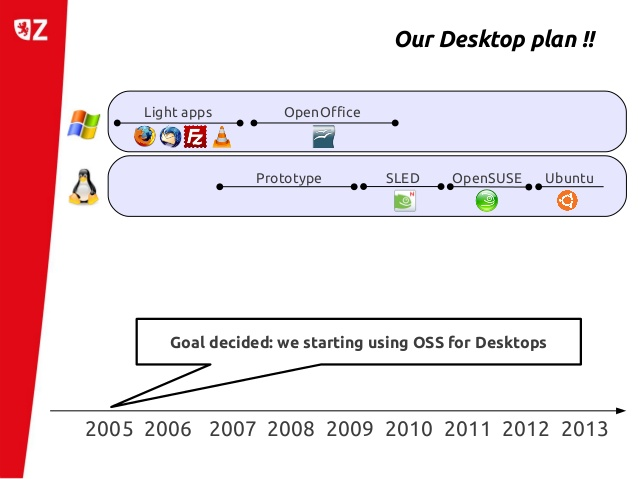
\includegraphics[scale=0.5]{img/zaragoza_desktopplan.png} 
       \caption[Zaragoza Desktop plan]{Zaragoza Desktop plan \protect\footnotemark}
         \end{figure}
     \footnotetext{Look at footnote \ref{planzaragoza}}


\item Phase 2: Office Applications – This phase allowed for the migration from Microsoft Office 97 to Open Office. The primary features in both office productivity suites are similar and contain similar functionality. There were issues present between MS Access and OpenOffice Database, given the fact that communication between the access documents was not possible; however, they were able to utilize Wine in GNU/Linux to complete the transfer. It was deemed the most important aspect of the migration process given the fact that all applications were utilized by all departments and the primary concern was not to interfere with the day to day operations of the departments, 
maintaining both quality and functionality. 
but recently they also started using LibreOffice, in combination with AZLinux12

\item Phase 3: Operating System – This phase consisted of the changeover in OS from Microsoft Windows XP to SUSE Linux Enterprise Desktop. Initially SuSE Linux Enterprise Desktop 10 was used in AZLinux 1, but this was changed to OpenSUSE 11.2 for AZLinux 2. SLED (SuSE Linux Enterprise Desktop) was the chosen application, given the fact that it had greater levels of integration with Novell Services (files, authentication, mail, etc.).
\end{itemize}
\textbf{Technical issues}
The city's IT department itself uses many more open source solutions, including for authentication (PAM\_LDAP), for digital certificates (FNMT) and for automatically migration tool to AZLinux (Win2Linux) and for system management they developed there own system (Migasfree\footnote{Migasfree is a Repository Manager where you put packages to distribute. These packages are responsible for performing the software configuration change, and must be created by each organization. Written in the Python programming language and using the Apache web server.}).

\subsection{Difficulties}

The difficulties that aroused were following:

\begin{enumerate}
\item Training gaps
It is hard to find qualified technicians in FLOSS in some specific field.
\item Low budget for additional costs, because there are costs associated with migration processes (training, acquisition of compatible hardware, etc.) these costs are not sufficiently understood.
\item Maintenance and Support. Many FLOSS projects implementation are carried out by individual initiative, without formal contracts to ensure their maintenance and support.
\item Lack of awareness of the importance of the FLOSS.
\end{enumerate}


\subsection{Cost}
In total, the project is expected to save as much as 15\% of the council's total IT budget, demonstrating an effective use of tax-payers' money to deliver better public services.

``\textit{The new open source strategy will reduce our software licensing costs by 50 percent potentially saving as much as \euro.500,000  per
year compared with our previous Microsoft solution.''}\footnote{Ricardo Cavero,Science and Technology CEO
Ayuntamiento de Zaragoza}.

\newpage

%---------------------------------------------------------------------------
\section {Munich, Germany  }
\begin{figure}[H]
\centering
    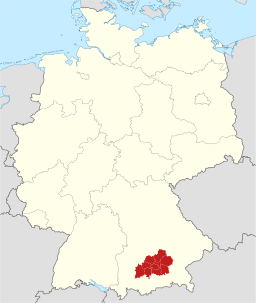
\includegraphics[scale=0.8]{img/munich.png} 
  \caption{Munich City}
  \label{Munich}
    \end{figure}

Munich, the capital of the federal state of Bavaria (Germany), has a population of approximately 1.23 million; it is the largest city in Bavaria and the third largest city in all of Germany, following on the heels of Berlin and Hamburg. The city of Munich has a network consisting of approximately 14,000 computers and approximately 16,000 users. The Linux distribution (distro) currently employed for a project sponsored by Munich’s city council is LiMux. The goal was total migration by January 2013 to FLOSS, allowing the city to achieve greater levels of independence from software distributors, client/server relations and native client software; the migration included more than 15,000 personal computers (PCs) and laptops of the city’s various public employees.

\subsection{The plan}
The goals of the city council included\footnote{\url{https://joinup.ec.europa.eu/elibrary/case/limux-it-evolution-open-source-success-story-never}}:
\begin{itemize}[itemsep=0ex]
\item FLOSS, including the use of office communication software based on open standards, for all desktop PCs in the municipality,
\item The ability to make, develop, and/or procure all administrative processes as platform-independent software,
\item The creation of a standardized IT platform that included all consolidated applications and data storage.
\end{itemize}
The migration process started in 2004 with the introduction of four specific goals for IT administrators:
\begin{enumerate}[itemsep=0ex]
\item The migration of all desktops from the Windows OS to the LiMux OS.
\item The migration of specialized administrative processes to the use of free, web-based, or native Linux solutions.
 \item The reduction of complexity through the consolidation of the number of software products utilized.
\item The transference of macros, templates, and forms to the new solution, introducing system management software deployment and a centralized sign-on process. 
\end{enumerate}
%---------------------------------------------------------------------------
\subsubsection{Training and  E-learning }
At the start of any migration, it is typically the department administrators that will need additional training, providing them with the opportunity of learning how to deploy and run the new software options. After the administrators and technical staff have received their training, it is then typically the responsibility of the project team to create an e-learning environment, one that will teach others about how to utilize the software. In this instance, the project team created ``LiMux Lemwelt'' (the LiMux learning world), allowing users to take advantage of the entire experience, providing users with the freedom to choose the different areas and software products that they wished additional training on, while allowing users to control the pace of their training. In 2007, the LiMux Lemwelt received the eurele, a European e-learning award, for its design and functionality. Workers who utilize this program were trained only when their specific area was up for migration, allowing them to smoothly transition, seamlessly applying what they learned within the training sessions to the real world setting.
\begin{figure}[H]
    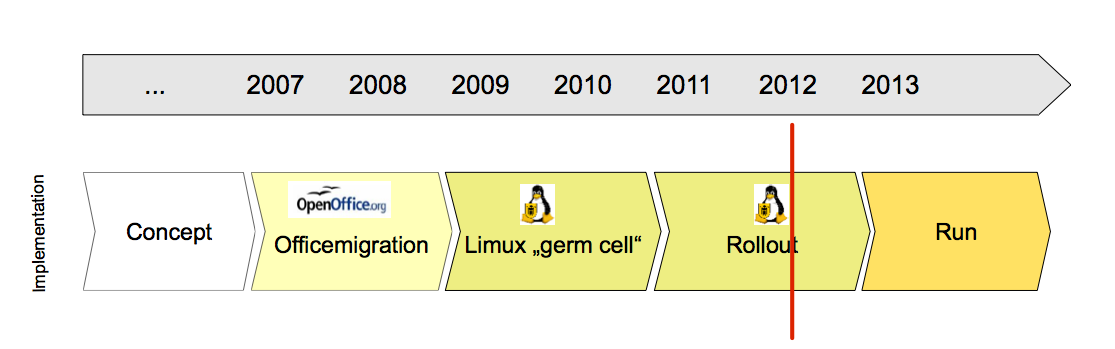
\includegraphics[scale=0.4]{img/timeline_limux.png}
 \caption  [Limux Timeline]{Limux Timeline © LiMux Project}  
\end{figure}
\subsection{Timeline}
The timeline determined for the implementation of this process was as follows:
\begin{itemize}
%---------------------------------------------------------------------------
\item 2001–2003: First plans and discussions based on the results of the city council of Munich votes.
\item 2003: project started.
\item 2005: The LiMux project started officially converting PCs.
\item 2008/2009: The first step, the complete switch to OpenOffice.org enabling the Open Document Format as standard format is done.
\item Late 2012: Initial goal of 12,000 Linux-based machines achieved.
\item  2013: Final acceptance documents signed, regular operations mode started, 14,800 machines migrated to Ubuntu Linux and LibreOffice.
\item December 2013: Munich open source switch completed successfully.

\end{itemize}
%---------------------------------------------------------------------------
\subsection{Cost}

Munich’s decision to leave Windows behind as their preferred and primary OS was not financially motivated, in spite of the fact that Munich indicated that the move to FLOSS allowed the city to save more than \$10 million In total, the LiMux project cost  \$23 million, as compared to the original  \$34 m  that was estimated it would cost to stay with Windows and MS Office. While HP created a report on behalf of Microsoft, that argued that the shift to FLOSS would cost three times as much as the official figures indicated, officials in Munich were able to show that the report was based off of a variety of flawed assumptions, among them being the overestimation of the number of staff it would take to accomplish the task.

 \begin{figure}
 \centering
     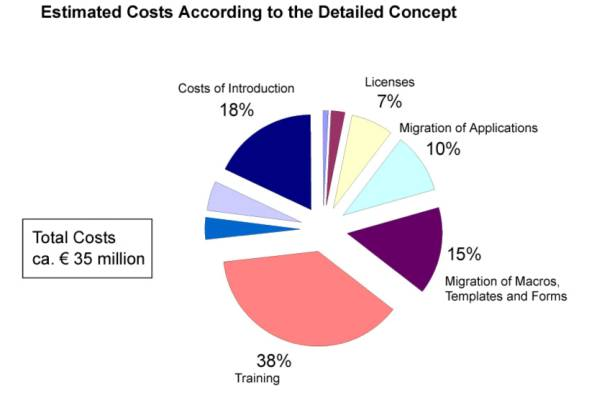
\includegraphics[width=0.86\textwidth]{img/cost_limux_estimates.png}
   \caption  [Limux cost estimates]{Cost Estimates According to the Detailed Concept \protect\footnotemark}  
   \label{fig:cost_limux_estimates}
 \end{figure}
 \footnotetext{source:\url{http://waste.informatik.hu-berlin.de/grassmuck/texts/limux.pdf`} }

Through a review of Figure \ref{fig:cost_limux_estimates}, it is possible to see that the final cost associated with training is the highest conceptualized cost estimate, according to LiMux – Free Software for Munich. 

\textit{``By combining the low costs and freedom of open source software with ongoing support for the hardware and applications we need, it was one of the critical elements to the success of this project. Most important was the backing of our politicians throughout the project.''}\footnote{Peter Hoffman, project manager for the City of Munich in \url{https://insights.ubuntu.com/2014/07/07/ubuntu-and-open-source-help-the-city-of-munich-save-millions/}}

\begin{figure}
\centering
    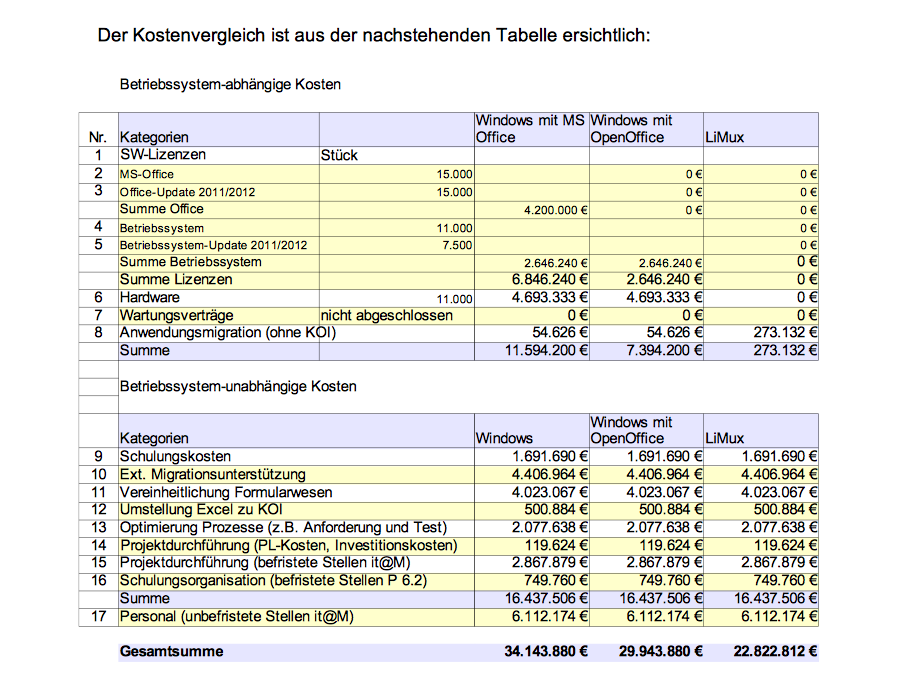
\includegraphics[scale=0.55]{img/limuxcost.png}
  \caption [Limux detailed cost]{Detailed figures of the LiMux project reveal differences from the original plan. Despite the economic success of LiMux, money has never been the driving factor. © Limux } 
\end{figure}
%---------------------------------------------------------------------------
\section {Largo, Florida}
\label{largo}
\begin{figure}[H]
\centering
    \includegraphics[scale=0.8]{img/Largo.png} 
  \caption{ Largo Florida City}
    \end{figure}
    
Largo is the third largest city in Pinellas County, Florida, USA.
The city of Largo has a population over 70,000 with over 650 employees utilizing FLOSS including the use of the Linux OS and many other FLOSS options. The initial migration to the use of FLOSS started with 650 employees being selected to utilize the new system. Starting in 1993, Largo implemented the use of a thin client, thick server architecture, accessible from 425 thin client workstations.

As the use of Microsoft Windows was considered expensive to purchase and maintain, Largo chose to implement a migration and upgrade strategy that utilized graphical workstation environments with thin client devices. The Largo architecture was running on open server and UnixWare. 

In 2000, problems and difficulties started to arise at the Santa Cruz operation\footnote{Santa Cruz Operation (SCO) was a software company based in Santa Cruz, California which was best known for selling three Unix variants for Intel x86 processors: Xenix, SCO UNIX (later known as SCO OpenServer), and UnixWare.}, the provider of the Open Server and UnixWare, the initial reason behind the decision of the Largo IT staff to start the replacement process. At this same time, Microsoft had just come out with Windows 2000, an OS that was full of bugs and difficult to maintain, not to mention highly costly; as an alternative, Largo chose to utilize Red Hat Inc.’s Linux Server options instead. The project started with 20 employees test running the new environment, and by the middle of 2001, Largo’s IT team was satisfied with the results.

 Largo’s environment serves 650 user accounts on a network of 400 computer devices. This network is served by two Compaq servers, with each server supporting approximately 220 users. KDE desktop environments are utilized by Largo’s staff. Opera and Netscape are the web browsers of choice, with Ximian based on the GNOME platform used as the primary email client, and Apache servers being utilized as additional application support.
 
 \subsection{Difficulties}
  Largo’s IT team succeeded in their experiment, but they believe that the primary barrier to greater acceptance of the use of FLOSS is the unbelieving nature of many that the software options are equal to or better than standard licensed programs.

\subsubsection*{Training users on Linux}
One of the biggest problems training new employees to switch from Windows PCs, to use Largo's Linux-based network. 
They are used to system crashes and network failures in Windows environments that they have trouble realizing, that all their files are stored on reliable servers -- with backups -- instead of on a desktop PC.

\textit{``There is also another, very human problem to overcome: that most people don't understand computers or software, but have memorized all the keystrokes and mouse-click patterns they need to get through the day, so the second they are given a new program they need to memorize a whole new set.''}\footnote{\url{http://www.largo.com/eGov/apps/document/center.egov?view=item;id=1793}} This can happen any time when new software is introduced in a workplace environment. But train people and answer users' questions will help new users to overcome this difficulties.

\subsection{Cost}
Systems administrators in Largo estimated that the use of Linux saves the city approximately \$1 m per year in hardware, software licensing, maintenance, and staffing costs, as of 2002. The IT staff looked at the possibility of continuing to utilize Microsoft Office, but ultimately decided that the total cost of installation, licensing, and maintenance could easily hit \$1.5 m over the course of a six year cycle, while the maintenance of OpenOffice during the same period would be roughly \$100,000\footnote{Look at the previous footnote} as in Figure~\ref{fig:Largo_cost}. 
\begin{figure}
\centering
    \includegraphics[scale=0.9]{img/largocost.png}   
 \caption[Largo Office Cost ]{Total Cost of Installation, Licensing, and Maintaining the Different Productivity Suites for a 6-year Cycle}
    \label {fig:Largo_cost}
\end{figure}


